\documentclass{article}

\usepackage{../acad} % https://github.com/rstanuwijaya/latex-template
\usepackage{xcolor}
\usepackage[]{minted}

\renewcommand{\sectionPrefix}{}

\title{PHYS5120 HW2}
\author{TANUWIJAYA, Randy Stefan \footnote{\LaTeX\ source code: \url{https://github.com/rstanuwijaya/hkust-computational-material/}}\\ (20582731) \\ rstanuwijaya@connect.ust.hk}
\affil{Department of Physics - HKUST}
\date{\today}

\definecolor{codegreen}{rgb}{0,0.6,0}
\definecolor{codegray}{rgb}{0.5,0.5,0.5}
\definecolor{codepurple}{rgb}{0.58,0,0.82}
\definecolor{backcolour}{rgb}{0.95,0.95,0.92}

\lstdefinestyle{mystyle}{
    backgroundcolor=\color{backcolour},   
    commentstyle=\color{codegreen},
    keywordstyle=\color{magenta},
    numberstyle=\tiny\color{codegray},
    stringstyle=\color{codepurple},
    basicstyle=\ttfamily\footnotesize,
    breakatwhitespace=false,         
    breaklines=true,                 
    captionpos=b,                    
    keepspaces=true,                 
    numbers=left,                    
    numbersep=5pt,                  
    showspaces=false,                
    showstringspaces=false,
    showtabs=false,                  
    tabsize=2
}
\lstset{style=mystyle}

\newcommand{\expc}[1]{\left<#1\right>}

\begin{document}
\maketitle
\begin{section}{Molecular Dynamics simulations of Lennard-Jones Argon}
The experimental data for Lennard-Jones argon:
$$
	\epsilon/k_B = \SI{119.8}{K}, \sigma = \SI{3.405}{\angstrom}, M = \SI{0.03994}{kg/mol}
$$

Use the ''md.py'' code provided here to run a MD simulation at the temperature $T = \SI{180}{K}$ and the density $\rho = \SI{1340}{kg/m^3}$. The simulation equilibrium should be at least 10 picoseconds.

\begin{enumerate}[1.]
	\item Calculate the temperature and the number density in reduced units.
	\begin{tcolorbox}[breakable]
		The unit of temperature in reduced unit is given by:
		\begin{align*}
			T & = \frac{T^{(\unit{K})}}{\epsilon/k_B} \\
			  & = \frac{\SI{180}{K}}{\SI{119.8}{K}}   \\
			  & = \SI{1.50}{}
		\end{align*}

		The unit of number density in reduced unit is given by:
		\begin{align*}
			\rho & = \frac{\rho^{(\unit{kg/m^3})}}{M/N_A \sigma^3} \\
			     & = \frac{\SI{1340}{kg/m^3}}{\SI{1680}{kg/m^3}}   \\
			     & = \SI{0.7976}{}
		\end{align*}
	\end{tcolorbox}

	\newpage
	\item Choose a proper time step. Plot kinetic energy, potential energy, and total energy versus simulation time. Are they stable?

	\begin{tcolorbox}[breakable]
		The reduced unit time is:
		\begin{align*}
			t_0 = \sigma \sqrt{m/\epsilon} = \sigma \sqrt{\frac{M}{N_A} \frac{1}{(\epsilon/k_B)k_B}} = \SI{2.157e-12}{s}
		\end{align*}

		Therefore, the total simulation time in reduced unit is:
		\begin{align*}
			t_{\text{total}} = \SI{10e-12}{s} / t_0 = \SI{4.63}{}
			\approx \SI{5}{}
		\end{align*}

		If we choose the total simulation steps to be 1000, then the time step is:
		\begin{align*}
			\Delta t = \frac{t}{1000} = 0.005
		\end{align*}

		We run the simulation using time step $dt=0.005$, using 1000 iterations of production run and 1000 iterations of equilibrium run. The results of equilibrium run are shown in Fig. \ref{fig:energy}. The energy is stable, and the potential energy is always negative. Note that we have also tried using different number of iterations (5000 and 10000), in which the results are similar.
		\begin{figure}[H]
			\centering
			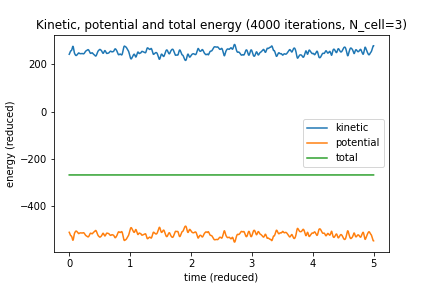
\includegraphics[width=0.8\textwidth]{images/energy.png}
			\caption{Energy versus simulation time.}
			\label{fig:energy}
		\end{figure}
		Note that the reduced unit of energy is given by: $ \epsilon = \SI{1.65e-21}{J}$ and the reduced unite of time is given by: $t_0 = \SI{2.157}{ps}$.
	\end{tcolorbox}

	\newpage
	\item Output unfolded coordinates as well as velocities in the Gromacs gro format: \url{http://manual.gromacs.org/archive/5.0.3/online/gro.html}. The length unit is nanometer (nm); the time unit is picosecond (ps); the velocity unit is nm/ps. A sample gro file for a MD trajectory is provided here. Save the trajectory on your machine (not canvas.ust.hk) and visualize it using the VMD software: \url{http://www.ks.uiuc.edu/ Research/vmd/}. In VMD, choose CPK as the drawing method (Graphics -> Representations -> Drawing Method) Attach one VMD screen shot in your PDF report. If your time step is very small, you do not need to write down every MD step, why? Use the saved gro file to do the following analyses.

	\begin{tcolorbox}[breakable]
		We have modified the \texttt{simulate()} function to output the coordinates and velocities in the Gromacs gro format for all of the 1000 frames. The output file is named \texttt{argon.gro}. The VMD screen shot is shown in Fig. \ref{fig:vmd}.
		\begin{figure}[H]
			\centering
			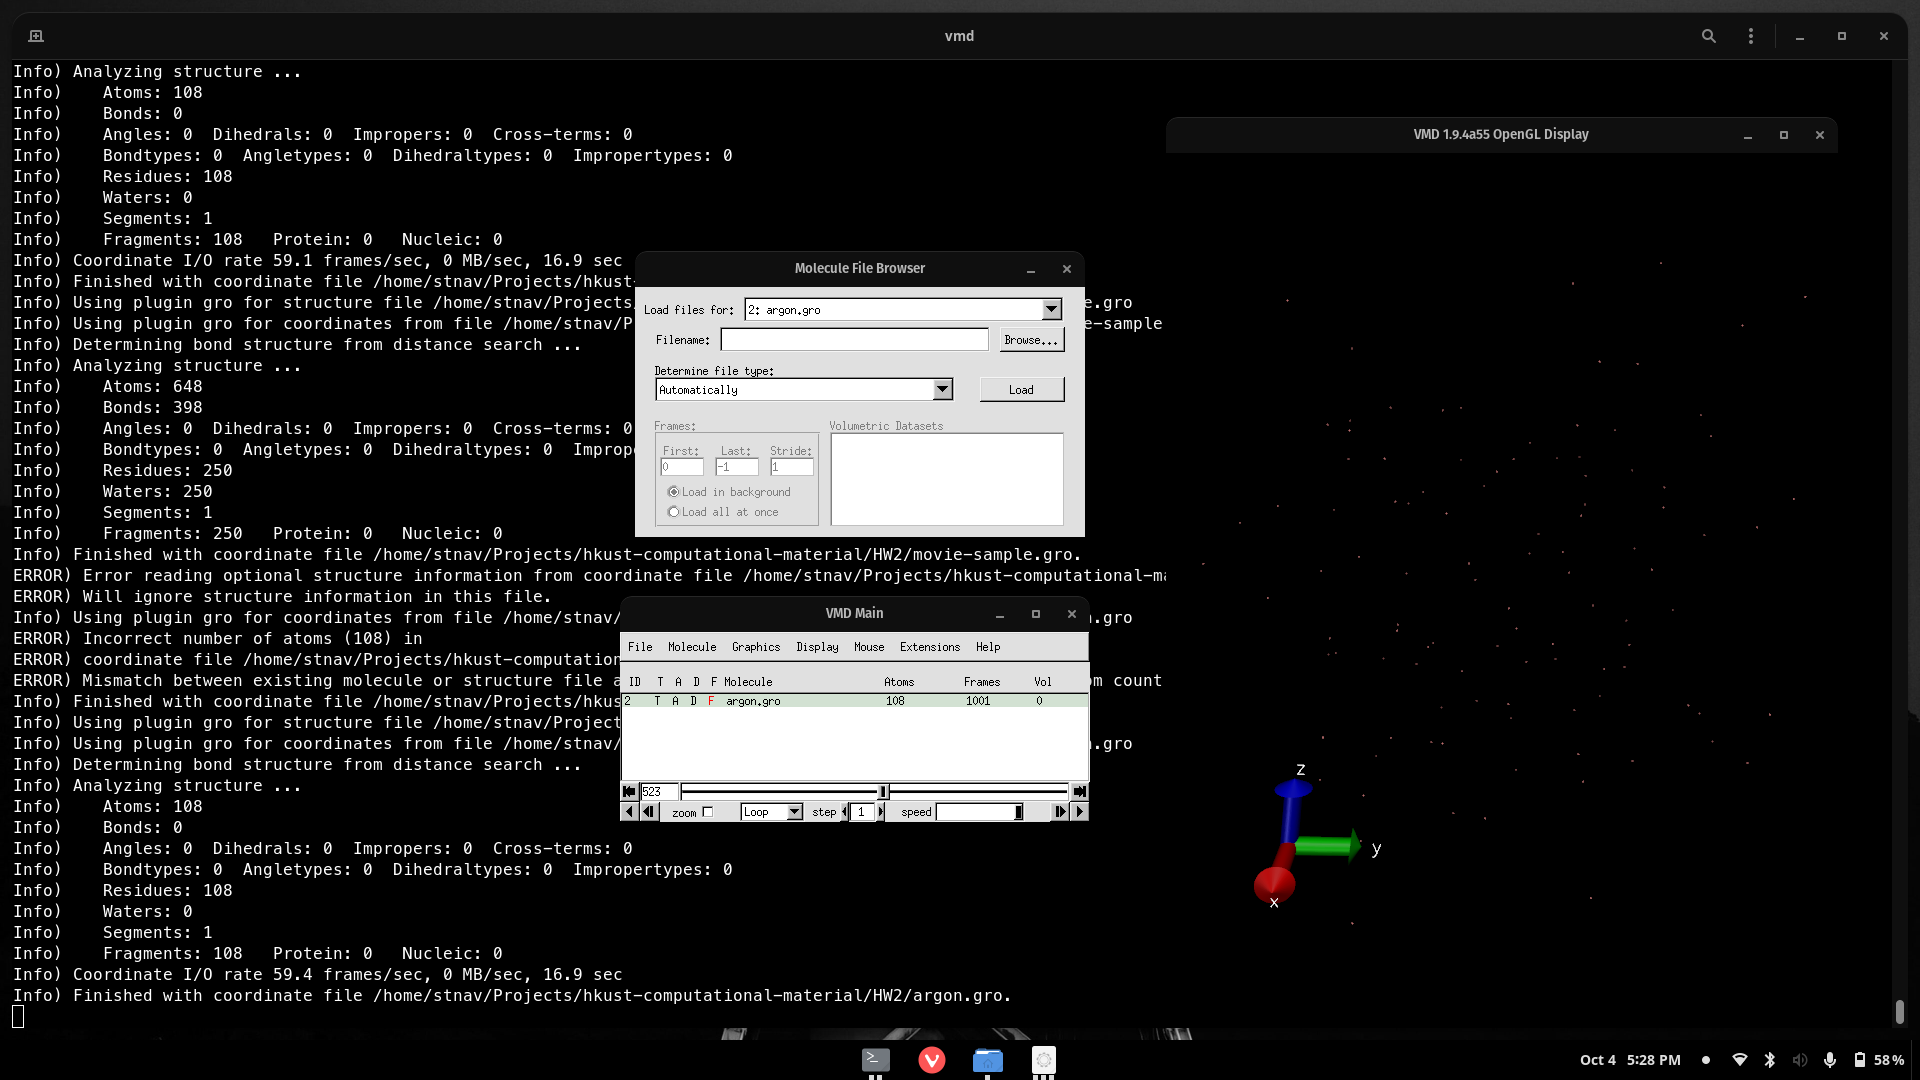
\includegraphics[width=0.8\textwidth]{images/vmd-argon-screenshot.png}
			\caption{Argon gas simulation using VMD.}
			\label{fig:vmd}
		\end{figure}

		In the case of using a smaller time step, not all of the frames are important as the particle movement will be slower and the file size grows linearly with the number of frames used in the Gromacs file.
	\end{tcolorbox}

	\newpage
	\item Write your own code to plot the radial distribution function of argon.

	\begin{tcolorbox}[breakable]
		Let $h(r)$ be the histogram of the (\textbf{minimum image}) distance between all particle pairs throughout all the frames in the simulation and $n(r) = h(r)*2/(N_\text{atoms} N_\text{frames})$ as the normalized distance histogram per atom per frame, i.e. $\sum n(r) = N$ The radial distribution is defined as:
		$$
			g(r + 0.5dr) = \frac{n(r)}{\rho dV} = \frac{n(r)}{4\pi \rho r^2 dr}
		$$

		The implementation can be found directly in the appendix.

		The radial distribution function of argon for ($N_\text{cell} = 3$) is shown in Fig. \ref{fig:radial_distribution}. As we can see from the figure, the plot is very similar to the one in the lecture notes for $r < L_\text{box}/2 \approx 2.57$ where the function suddenly decays. To obtain the radial distribution for larger $r$, we can try to increase the simulation box size by increasing $N_\text{cell}$ to 4 or 5. However, this will increase the simulation time significantly.

		\begin{figure}[H]
			\centering
			\begin{minipage}{0.45\textwidth}
				\centering
				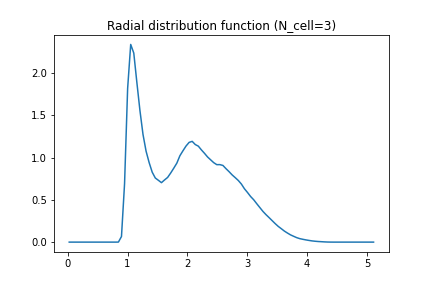
\includegraphics[width=\linewidth]{images/g_r(N_cell=3).png}
			\end{minipage}
			\begin{minipage}{0.45\textwidth}
				\centering
				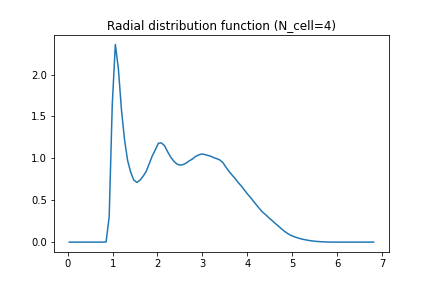
\includegraphics[width=\linewidth]{images/g_r(N_cell=4).png}
			\end{minipage}
			\caption{Radial distribution of argon for $N_\text{cell} = 3$ and $N_\text{cell} = 4$.}
			\label{fig:radial_distribution}
		\end{figure}
	\end{tcolorbox}

	\newpage
	\item Calculate the diffusion constant (coefficient) using both the Einstein relation 1 and the Green-Kubo method. Are the two results consistent? Because of periodic boundary conditions, we have folded and unfolded coordinates. Which one should be used to calculate the mean squared displacement? Why?

	\begin{tcolorbox}[breakable]
		Recall the Einstein relation:
		$$
			D = \frac{1}{6 N_\text{atom}} \sum_i^{N_\text{atom}}
			\frac{d[r_i(t+dt) - r_i(t)]^2}{dt}
		$$
		And the Green-Kubo relation:
		$$
			D = \frac{1}{3 N_\text{atom}} \int \sum_i^{N_\text{atom}}
			x[v_i(t+dt) \cdot v(t)] dt
		$$
		Note that for Einstein diffusion coefficient, the coordinates system used should be the unfolded coordinates. However, since the simulation uses the folded coordinates, we can see there will be some discrepancy with the diffusion constant found using the Green-Kubo relation.

		The results of the velocity autocorrelation for each frames obtained using the two methods are shown in Fig. \ref{fig:V_ac}. We can observe that the two results are consistent but the autocorrelation obtained using Einstein method is scaled by a factor of $\sim 0.5$. The corresponding diffusion constant given by the two methods are:
		\begin{align*}
			D_\text{einstein}   & = 3.716 \\
			D_\text{green-kubo} & = 7.417
		\end{align*}
		as we have argued above, the correct diffusion constant should be $D_\text{green-kubo}$.

		\begin{figure}[H]
			\centering
			\begin{minipage}{0.45\textwidth}
				\centering
				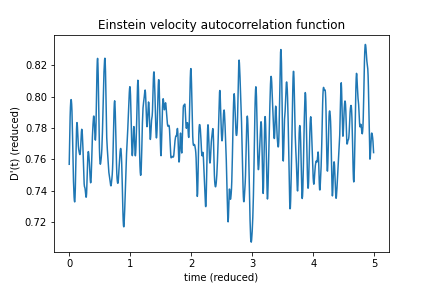
\includegraphics[width=\linewidth]{images/V_ac_einstein.png}
			\end{minipage}
			\begin{minipage}{0.45\textwidth}
				\centering
				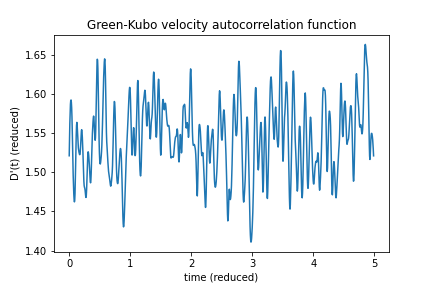
\includegraphics[width=\linewidth]{images/V_ac_gkb.png}
			\end{minipage}
			\caption{Velocity autocorrelation for each frames obtained using the Einstein relation and the Green-Kubo relation.}
			\label{fig:V_ac}
		\end{figure}
	\end{tcolorbox}
\end{enumerate}
\end{section}

\newpage
\begin{section}{Appendix}
\begin{enumerate}
	\item Python code for MD simulation
	\begin{minted}[mathescape,
		linenos,
		numbersep=5pt,
		gobble=8,
		frame=lines,
		framesep=2mm]{python}
        import numpy as np
        import matplotlib.pyplot as plt
        from math import sqrt, pi
        from itertools import product

        sigma = 0.3405  # nm
        t0 = 2.157  # ps
        n_bins = 100

        T_0 = 1.50  # temperature
        rho = 0.7976  # density of Argon in reduced units
        # T_0 = 0.71  # temperature
        # rho = 0.844  # density of Argon in reduced units

        n_frames = 1000
        dt = 5/n_frames  # time step size
        N_cell = 4  # number of fcc unitcells in one direction
        N = 4 * N_cell ** 3  # the total number of particles in the system
        L_box = (N / rho) ** (1 / 3.0)  # length of the whole simulation box
        L_cell = L_box / N_cell  # length of a unitcell
        F = np.zeros((N, N, 3))  # matrix that contains all forces
        ind = np.triu_indices(N, k=1)  # indices of upper triangular matrix


        def IC_pos(N_cell, L_cell):
            '''
            use fcc structure to initilize positions
            '''
            pos = [[[x,  y, z],
                    [x, 0.5 + y, 0.5 + z],
                    [0.5 + x, y, 0.5 + z],
                    [0.5 + x, 0.5 + y, z]]
                    for x, y, z in product(range(N_cell), range(N_cell), range(N_cell))]
            pos = np.array(pos).reshape((-1, 3))
            return pos * L_cell


        def IC_vel(N):
            '''
            Maxwell-Boltzman distribution is a normal distribution
            '''
            vel = np.sqrt(T_0) * np.random.randn(N, 3)
            vel -= np.average(vel, axis=0)
            return vel


        def find_force(pos, L_box=L_box):
            '''
            Minimum image convention. 
            '''
            r_vec = pos[ind[0]] - pos[ind[1]]
            r_vec = r_vec - np.rint(r_vec / L_box) * L_box
            r_sq = np.sum(r_vec**2, axis=1)
            F_vec = -(48 / r_sq ** 7 - 24 / r_sq ** 4)[:, None] * r_vec
            F[ind[0], ind[1]] = F_vec
            pot = np.sum(4 / r_sq ** 6 - 4 / r_sq ** 3)
            P = np.sum(F_vec * r_vec)
            return np.sum(F, axis=0) - np.sum(F, axis=1), pot, P


        def time_step(pos, vel, F):
            vel += 0.5 * F * dt
            pos = pos + vel * dt
            pos_folded = np.mod(pos, L_box)
            # pos = np.mod(pos + vel * dt, L_box) # why both pos and pos_folded?
            F, pot, P = find_force(pos_folded)

            vel += 0.5 * F * dt
            kin = 0.5 * np.sum(vel**2)
            return pos, vel, F, pot, kin, P


        def min_dist(r):
            if r > L_box/2:
                return r - L_box
            elif r < -L_box/2:
                return r + L_box
            else:
                return r


        def simulate(f, h_r, bins, drs, dvs):
            kins, pots, Ps = [], [], []
            pos = IC_pos(N_cell, L_cell)
            prev_pos = pos
            vel = IC_vel(N)
            prev_vel = vel
            dr, dv = 0, 0
            F = find_force(pos)[0]
            for i in range(2*n_frames):
                pos, vel, F, pot, kin, P = time_step(pos, vel, F)
                if i > n_frames:  # production run
                    kins.append(kin)
                    pots.append(pot)
                    Ps.append(P)

                    SI_pos = pos*sigma
                    SI_vel = vel*sigma/t0

                    f.write('MD of 1 Argon t=%10.5f\n' % (i * dt * t0))
                    f.write('%5d\n' % (N))
                    for j in range(N):
                        f.write('%5d%-5s%5s%5d%8.3f%8.3f%8.3f%8.4f%8.4f%8.4f\n' %
                                (j, 'ARGON', 'Ar', j,
                                    SI_pos[j][0], SI_pos[j][1], SI_pos[j][2],
                                    SI_vel[j][0], SI_vel[j][1], SI_vel[j][2]))
                    f.write('%10.5f%10.5f%10.5f\n' %
                            (L_box*sigma, L_box*sigma, L_box*sigma))

                    r_vec = pos[ind[0]] - pos[ind[1]]
                    r_vec = r_vec - np.rint(r_vec / L_box) * L_box
                    r_sq = np.sum(r_vec**2, axis=1)
                    h_r += np.histogram(np.sqrt(r_sq), bins)[0]

                    drs.append(np.average(np.sum((pos-prev_pos)**2, axis=1)))
                    dvs.append(np.average(np.sum((vel*prev_vel), axis=1)))
                else:  # equillirum run
                    vel *= np.sqrt(N * 3 * T_0 / (2 * kin))
                prev_pos = pos
                prev_vel = vel

            return np.array(kins), np.array(pots), np.array(Ps)


        # The simulation starts here
        if __name__ == "__main__":
            h_r = np.zeros(n_bins)
            bins = np.linspace(0, L_box, n_bins+1)

            drs = []
            dvs = []

            with open('argon.gro', 'w') as f:
                kins, pots, Ps = simulate(f, h_r, bins, drs, dvs)
            times = np.arange(len(kins)) * dt
            T = np.mean(kins * 2 / (3 * N))  # temperature
            P = 1 - np.mean(Ps) / (3 * N * T) - 16 * np.pi * \
                rho / (3 * T * L_box**3)  # compressibility factor
            P = P * T * rho  # pressure here
            # print(T, P)  # how about thermal fluctuation?
            # print(pots)

            # plot the energy vs time results
            plt.plot(times, kins)
            plt.plot(times, pots)
            plt.plot(times, kins+pots)
            plt.legend(['kinetic', 'potential', 'total'])
            plt.xlabel('time (reduced)')
            plt.ylabel('energy (reduced)')
            plt.title(f'Kinetic, potential and total energy ({n_frames} iterations)')
            plt.savefig('images/energy.png')
            plt.show()

            n_r = (h_r*2/((N-1)*(n_frames-1)))
            g_r = n_r/(4/3*pi*((bins[1:])**3 - (bins[:-1])**3)*rho)
            plt.plot(bins[:n_bins]+(bins[1]-bins[0])/2, g_r)
            plt.title(f'Radial distribution function (N_cell={N_cell})')
            plt.savefig(f'images/g_r(N_cell={N_cell}).png')
            plt.xlabel('r (reduced)')
            plt.ylabel('g(r)')
            plt.show()

            V_ac_einstein = np.array(drs)/(6*dt**2)
            V_ac_gkb = np.array(dvs)/3

            D_einstein = np.sum(V_ac_einstein)*dt
            D_gkb = np.sum(V_ac_gkb)*dt
            plt.plot(times, V_ac_einstein)
            plt.title('Einstein velocity autocorrelation function')
            plt.xlabel('time (reduced)')
            plt.ylabel('D\'(t) (reduced)')
            plt.savefig('images/V_ac_einstein.png')
            plt.show()

            plt.plot(times, V_ac_gkb)
            plt.title('Green-Kubo velocity autocorrelation function')
            plt.xlabel('time (reduced)')
            plt.ylabel('D\'(t) (reduced)')
            plt.savefig('images/V_ac_gkb.png')
            plt.show()

            print('Average Einstein diffusion coefficient', D_einstein)
            print('Average Green-Kubo diffusion coefficient', D_gkb)
            print('Ratio', D_gkb/D_einstein)
		\end{minted}

	\item Compiling VMD from source on linux
	
	Just writing here in case I forget how to do it again or other students asks you in the future. The VMD on Windows has an installer, but on linux you have to compile it from source. Luckily, I found a tutorial on youtube on how to do it: \url{https://www.youtube.com/watch?v=7YA7IyxrxKw}, but it requires root permission to install. In short:
	\begin{enumerate}
		\item Download the source code from \url{https://www.ks.uiuc.edu/Research/vmd/}
		\item Run \texttt{./configure}
		\item \texttt{cd src \&\& sudo make install}
		\item VMD should be installed systemwide to \texttt{/usr/local/bin/vmd}
	\end{enumerate}
\end{enumerate}
\end{section}
\end{document}
